\chapter{File Feedrate Control}
\label{chapter5}
\section{Problem Definition and the Proposed Method}
\subsubsection{Problem Definition}
\hspace*{6mm}Instrument fracture is a potential crisis for endodontic treatment. If a dentist improperly operates an endodontic file, it will increase the possibility of instrument fracture. Most largely, the instrument fracture will happen while a file is inserted into the one-third place far from the root apex. It is barely possible to take out in a small root canal. Removal of broken files is technically tricky, so it is critical to reducing the probability of the instrument fracture.
\par

There is a technical solution to detect a status of a file. When a file suffers a force, it will lead to the crystalline phase transformation. However, it can only be observed from a microscope. It is impracticable to usually monitor it during the surgery. Previous literature shows there are two main causes of fractured files are torsional fracture and flexural fatigue, which account for 55.7\% and 44.3\% separately\cite{SATTAPAN2000161}. Therefore, we can reduce the torque a file bears to prevent the instrument fracture.
\subsubsection{File Property}
\hspace*{6mm}To protect the endodontic file from fracturing, we need to be familiar with its physical property and its correct operations. We delve into the physical properties of an endodontic file. A file is made of alloys of Nickel and Titanium, which is a superelastic material. The Ni-Ti file has significantly more elastic and incorruptible properties. This feature allows it to bend when inserted into a curve root canal and thereby reduces the possibility of stuck.
\begin{figure}[htbp]
\begin{center}
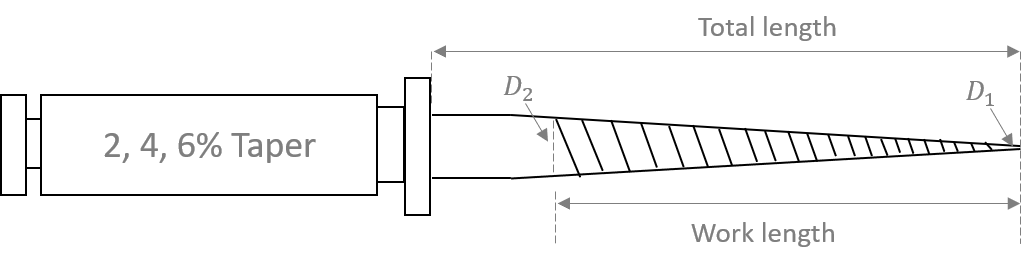
\includegraphics[width=1\linewidth]{Images/Endodontic_File.png}
\caption{The illustration of an endodontic file
}\label{fig: Endodontic File}
\end{center}
\end{figure}	
\par
In Fig \ref{fig: Endodontic File}, an endodontic file is illustrated. There are four types of total length - $21$, $25$, $28$, and $31$ mm. They all have the same work length - $16$ mm. Each file has their own number such as $\#15, \#20, \#25, \cdots, \#40$ shown as Fig \ref{fig: files}, which represent the diameter of files. Take a $\#15$ file with $2\%$ taper for example,
\par\noindent
the diameter of the tooltip $D_1$ is
\begin{equation*}
\begin{split}
15/100=0.15 \text{ (mm)}
\end{split}
\end{equation*}
and the diameter at the end of the work length $D_2$ is
\begin{equation*}
\begin{split}
0.15 + 16 \cdot 6\% = 1.11 \text{ (mm)}
\end{split}
\end{equation*}
\par
\begin{figure}[htbp]
\begin{center}
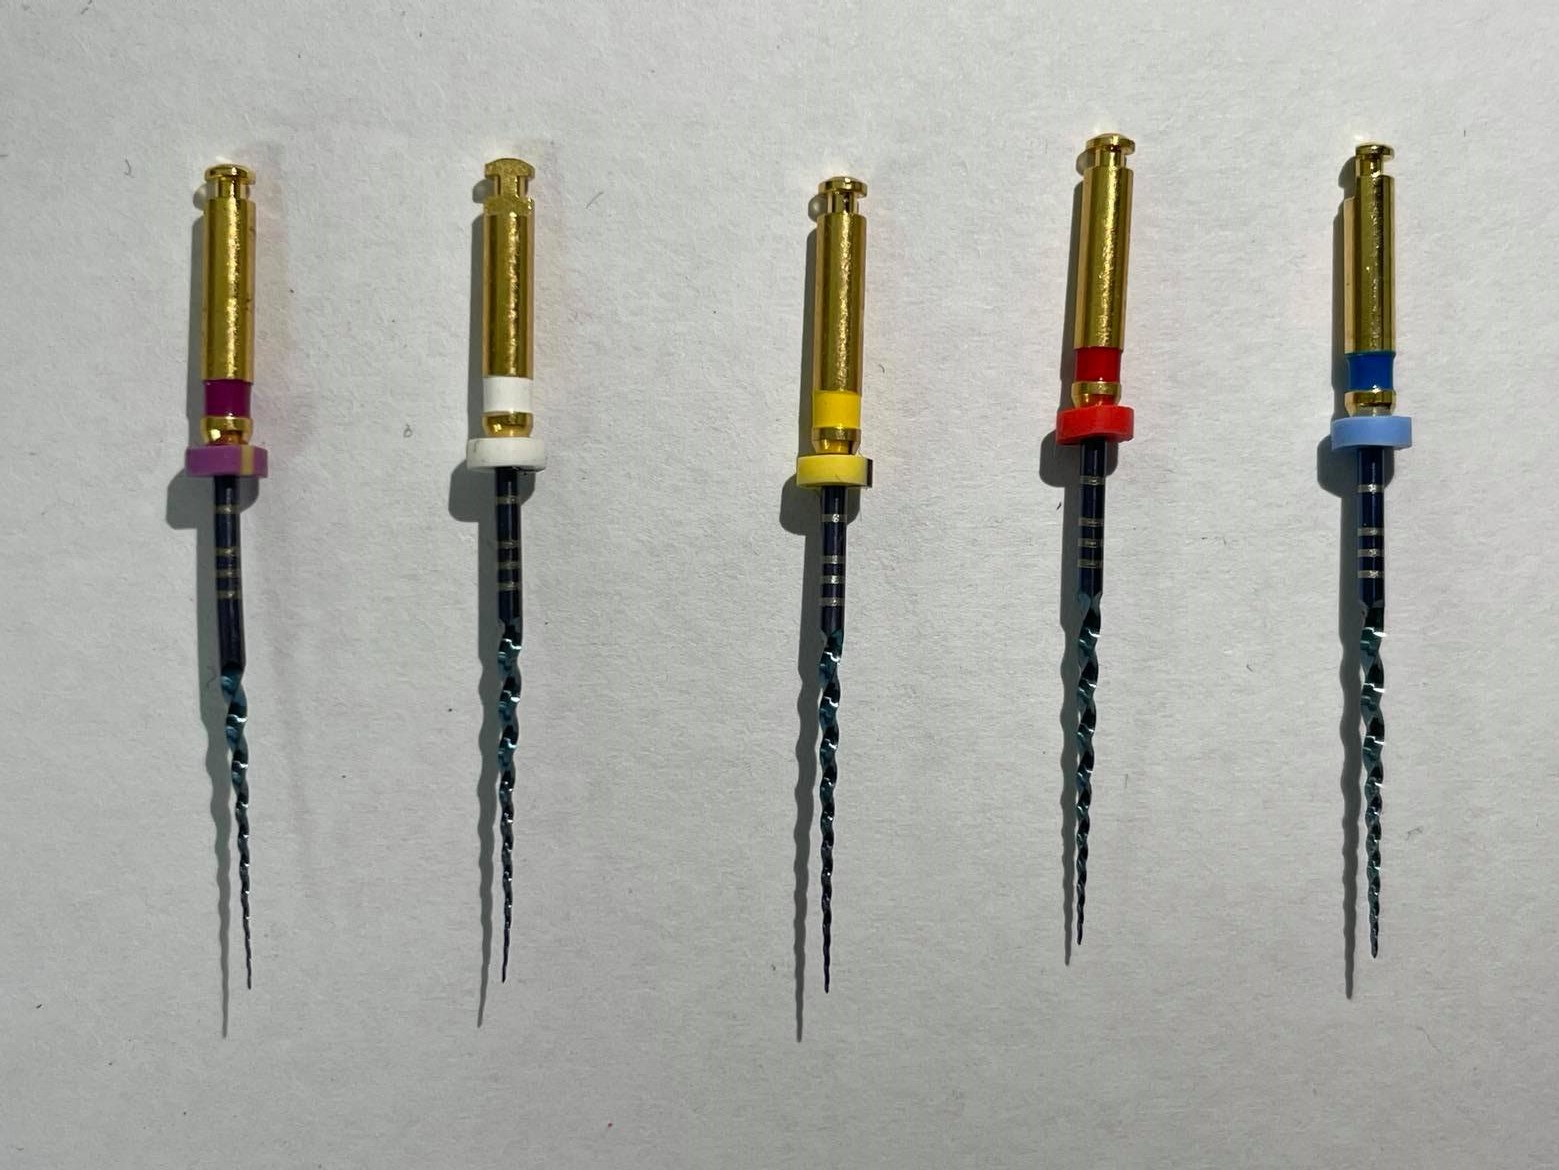
\includegraphics[width=0.7\linewidth]{Images/files.jpg}
\caption{Endodontic files with different diameters
}\label{fig: files}
\end{center}
\end{figure}	
\subsubsection{The Proposed Method}
\hspace*{6mm}In order to protect an endodontic file from fracturing, we need to reduce the file torque. The easiest and most effective way to solve this issue would be monitoring the torque which the file is enduring. Therefore, we implement a torque monitoring system on DentiBot. We utilize current feedback to keep track of the torque. An increase in the current of the motor is indicative of the contact resistance of the file. Also, We propose two approaches to release the file torque. One is inverse rotation control discussed in section \ref{sec:Inverse Rotation Control} and the other is feed control discussed in section \ref{sec:Feed Control}, they are both efficient ways to release the file torque. Once the torque of the file is in excess of a threshold, it will inversely rotate or decline the feedrate to release torque. 
\subsubsection{How to measure the file torque}
\hspace*{6mm}There are two approaches to measure the file torque. One is detecting the current of motor which drives the file rotation to estimate the file torque. The other is directly obtained from the F/T sensor after changing the reference frame to the tool frame. 
\par
Here we delves into the first method - detecting the current of motor to estimate the file torque. A motor can be modelled as an RL circuit. In this way, we can get the following formula 
\begin{equation}
\begin{split}
V = R \cdot I + L  \cdot \frac{\mathrm{d}I}{\mathrm{d}t} + \varepsilon
\end{split}
\end{equation}
where $V$ represents the input voltage, $I$ represents the input current, and $\varepsilon $ represents the back EMF produced by the motor motion.
\par
Since the value of the inductance of DC motor is small, we ignore the inductance term L. After transposition, we can get the following relation between the current and the back EMF.
\begin{equation}
\label{eq:current and the back EMF}
\begin{split}
I = \frac{I - \varepsilon}{R}
\end{split}
\end{equation}
\par\noindent
The back EMF produced by the motor is dependent upon the motor constant $K$, shown as the following equation.
\begin{equation}
\label{eq: the back EMF}
\begin{split}
\varepsilon  = K \cdot \frac{\mathrm{d}\theta (t)}{\mathrm{d}t} = K \cdot \omega (t)
\end{split}
\end{equation}
\par
When the file encounters resistance during the drilling procedure, the rotating speed of the motor would slow down. With the Equation \ref{eq:current and the back EMF} and \ref{eq: the back EMF} we can infer that the back EMF would decrease, and the current would increase.
Also, we have the relation between the current and torque
\begin{equation}
\begin{split}
T_m = K_m  \cdot \ I
\end{split}
\end{equation}
where $k_m$ represent the torque constant of a motor.
\par\noindent
The maximum torque a root canal file can bear is $6.20$ Ncm ($62.0$ mNm) \cite{boessler2009effect}. Therefore, we can derive the following inequality.
\begin{equation}
\begin{split}
T_m \cdot \mathrm{GR} < 62 \text{ (mNm)}
\end{split}
\end{equation}
where $\mathrm{GR}$ is gear ratio of gearbox mounted on a motor.
\par
Hence, we can set a current threshold based on the following condition. 
\begin{equation}
\begin{split}
I_{max} < \frac{62}{\mathrm{GR} \cdot K_m}
\end{split}
\end{equation} 
In realistic implementation, $\mathrm{GR}$ is $67$ and $K_m$ is $16 \text{mNm/A}$
\section{Inverse Rotation Control}
\label{sec:Inverse Rotation Control}
\hspace*{6mm}This proposed approach is an effective way to protect endodontic file from fracturing. Also, it can remove root debris cut by file and prevent file from getting stuck in root. Once the current of the file exceeds the specific threshold, it will inversely rotate for 90 degrees to release torque and then continue drilling in the original direction. Before designing the DentiBot, we have validated this function with the prototype of DentiBot shown as Fig \ref{fig: prototype}. This prototype is a drilling system mounted on a magnetic stand. The modified handpiece, a hand-held dental electric device, with a single axis mechanism can validate the inverse rotation control. 
\begin{figure}[htbp]
\begin{center}
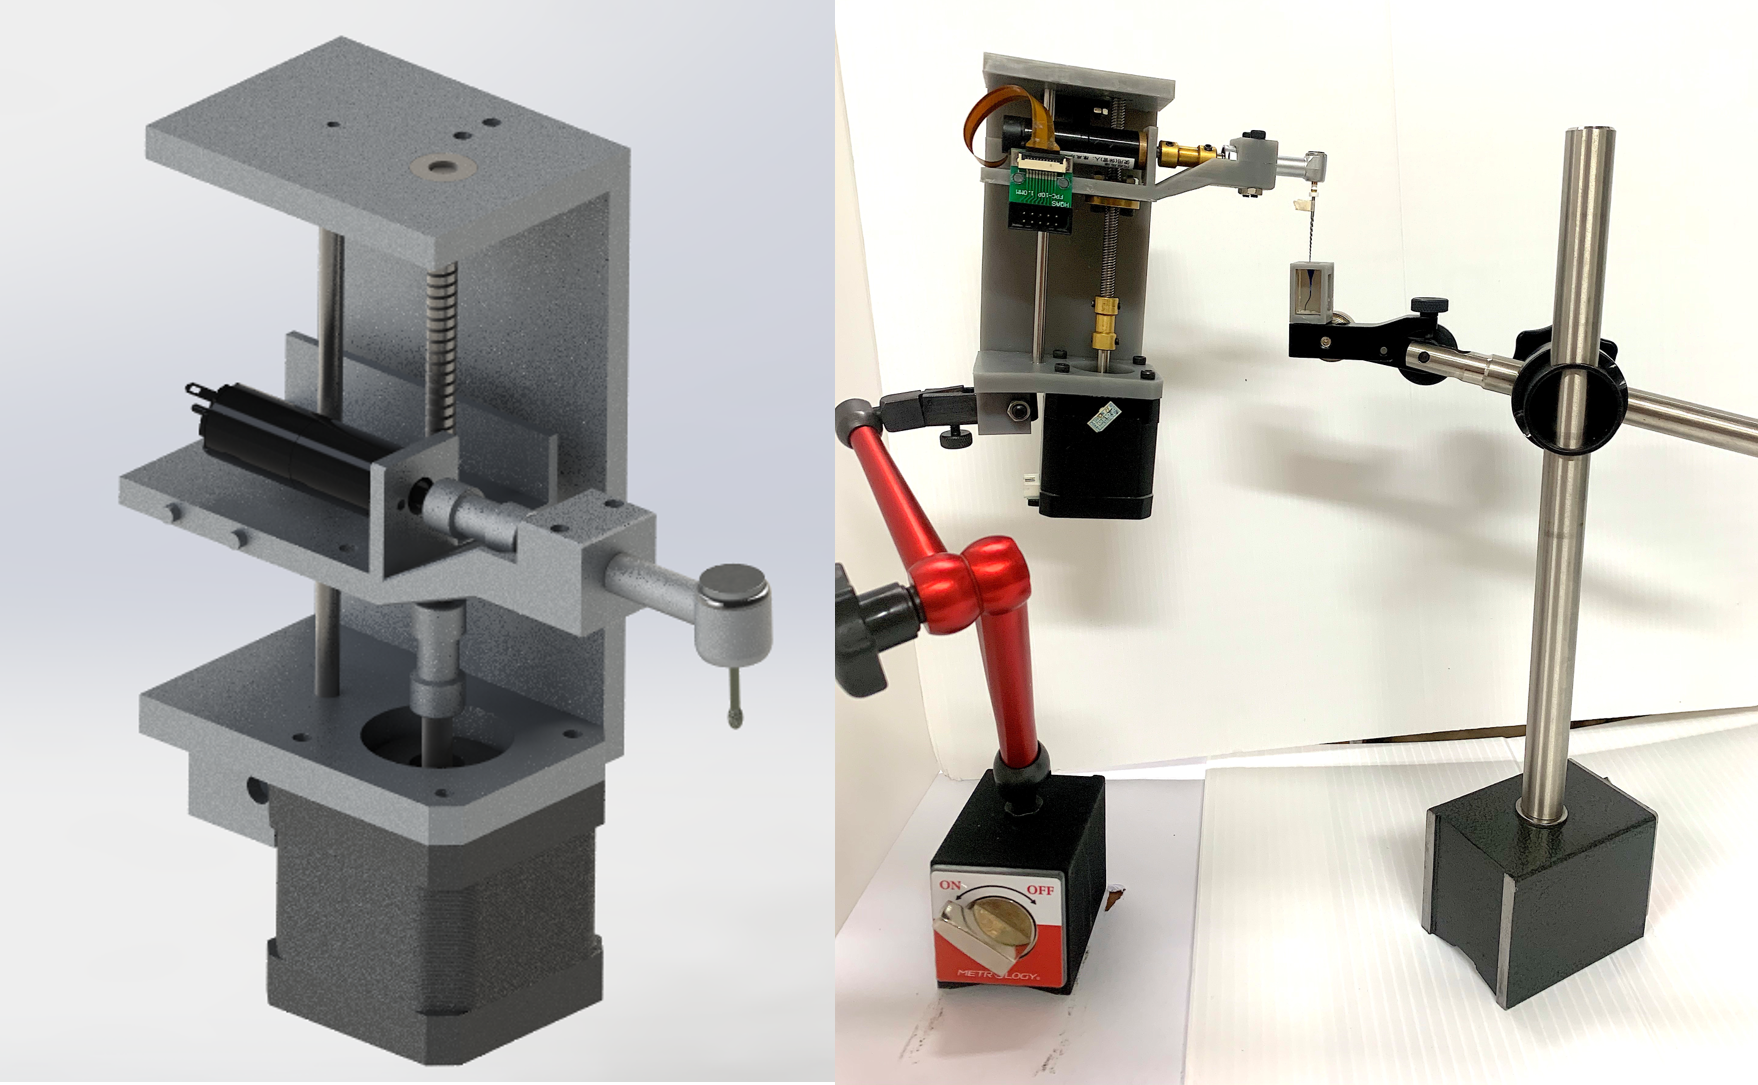
\includegraphics[width=0.9\linewidth]{Images/Prototype.png}
\caption{The prototype of DentiBot. A single z-axis manipulator with a modified handpiece}
\label{fig: prototype}
\end{center}
\end{figure}	
\par
In Fig \ref{fig: inverse_rotation}, a motion planning is designed to perform the drilling procedure. The root canal is divided into several sections to be cleaned. In the beginning, the robot moves to the start point and then repetitively drills one section back and forth at least ten times until the current feedback decrease under the specific threshold. If the torque exceeds the threshold, the endodontic file will inversely rotate for $90$ degrees to release the torque and then drill the same section again. After one section is cleaned thoroughly, the drilling file will move to the next section. Every section will be cleaned for at least $10$ rounds. If there is reverse rotation, it will be more than $10$ rounds. When to finish is contingent on whether the endodontic file reaches the final section.
\begin{figure}[htbp]
\begin{center}
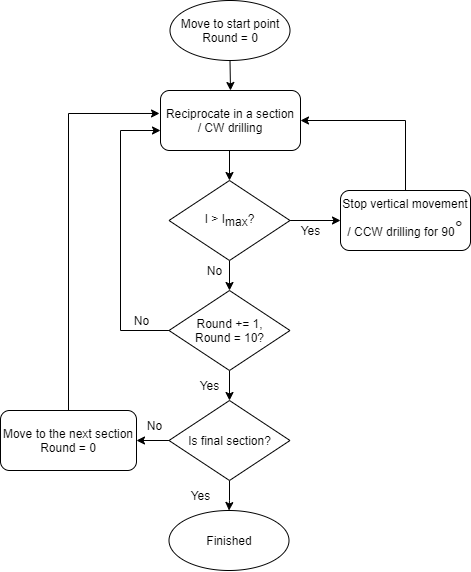
\includegraphics[width=0.8\linewidth]{Images/inverse_rotation.png}
\caption{Motion planning of Inverse Rotation Control with the prototype of DentiBot.}
\label{fig: inverse_rotation} 
\end{center}
\end{figure}
\par
In conclusion, by the preliminary experiment with the prototype of DentiBot, it has been proved that the inverse control rotation is an effective approach to reduce the torque. Therefore, we can detect the current to estimate the torque and inversely rotate the motor if the current exceeds the threshold current. 
\section{Feedrate Control}
\label{sec:Feed Control}
\hspace*{6mm}As mentioned above, we have validated the inverse rotation control with the prototype. However, inverse rotation control is just mimicking a dentist to perform endodontic treatment. It is still time-consuming. Hence, the other method - feed control is proposed to improve this problem. Note that this method can only be valid with DentiBot instead of its prototype because admittance control will be involved. Previous literature which dedicate to a form drilling with torque control is similar to our root drilling \cite{boessler2009effect}. Regulating the feedrate to control the torque is a effective way to reduce time. 
\begin{equation*}
\begin{split}
V\!f = f \cdot N
\end{split}
\end{equation*}
where $V\!f$ denotes feedrate. $f$ denotes feed per revolution. $N$ denotes spindle speed (rpm).
\par
As the above equation, regulating the feed and spindle can both affect feedrate. Refer to the previous literature, we set the spindle speed a constant ($60$ rpm) and the feed a variable. Therefore, we regulate the feed instead of the spindle speed to determine the feedrate. A similar control scheme for our root drilling is proposed and shown as Fig \ref{fig: feedrate_control}.
\begin{figure}[htbp]
\begin{center}
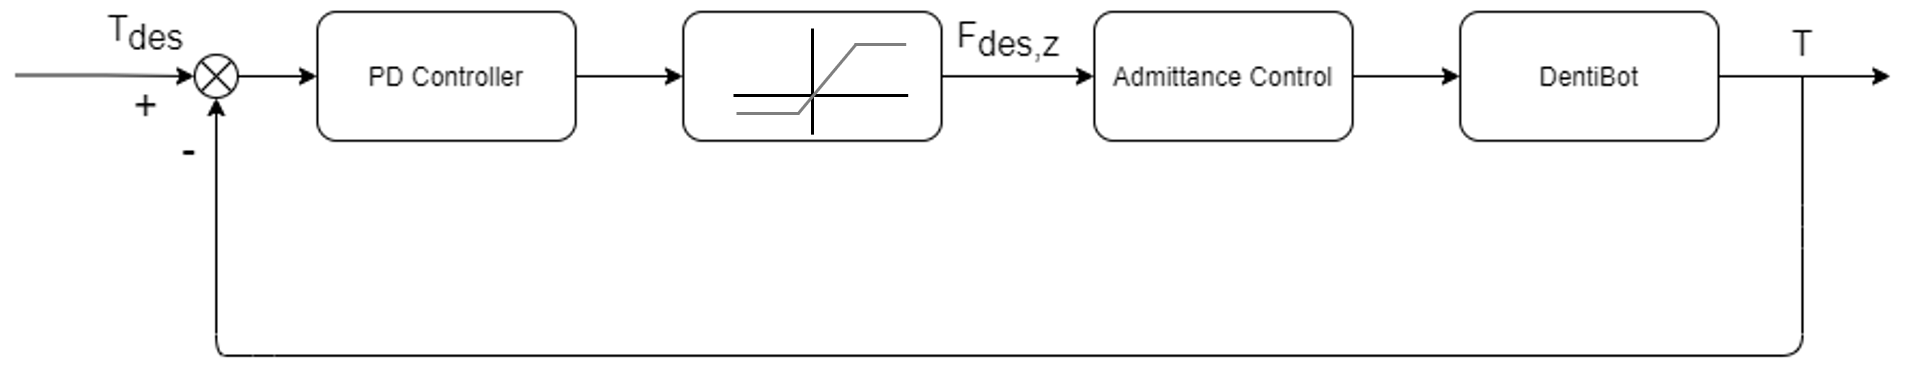
\includegraphics[width=1\linewidth]{Images/feedrate_control.png}
\caption{Control scheme of Feedrate Control with the DentiBot.}
\label{fig: feedarte_control}
\end{center}
\end{figure}
\par
The input is $\mathrm{T_{des}}$ and the feedback is $\mathrm{T}$. $f^*_z$ will be determined by the difference of $\mathrm{T_{des}}$ and $\mathrm{T}$ via a PD controller. Here we use a minimum and maximum saturation to bound $f^*_z$ and then output $f_z$. $f_z$ is the input of admittance control and is relevant to  the feed of z-axis. With the admittance control of DentiBot, DentiBot can move along with the tool because $f_z$ is related to the moving direction, which is exactly the insertion of tool. In conclusion, the feedrate can be regulated by the torque. When the file torque increases , DentiBot will decrease its moving velocity to control the increase rate of file torque.  It is worth noting that we combine admittance control into this approach. This feature not only provides the moving direction, but also tracks the root path and patient moving. Once the F/T sensor detects the extra value different from $[0\ 0\ f_z\ 0\ 0\ 0]$, the DentiBot will move to the correspond position and orientation. Moreover, because the z-orientation should be only acted by the file rotation driven by the motor, it is important to turn off z-orientation of admittance control by setting the parameter $b_6$ of admittance control as a large value.

\par
Entire flow chart is shown in Fig \ref{fig: feedrate_control_fc}. Considering the realistic condition, Dentibot judges whether patient moving happens by checking whether $||(f_x,f_y,f_z)||$ is larger than $1.5$ N. File rotation will stop and $f_z$ will be zero to stop moving when the value is more than $1.5$ N, then DentiBot can keep track of the patient moving. If not, DentiBot will continue drilling with feedrate control until the tooltip reaches the apex of root. The feasibility is proven in experiment 1-3.
\begin{figure}[htbp]
\begin{center}
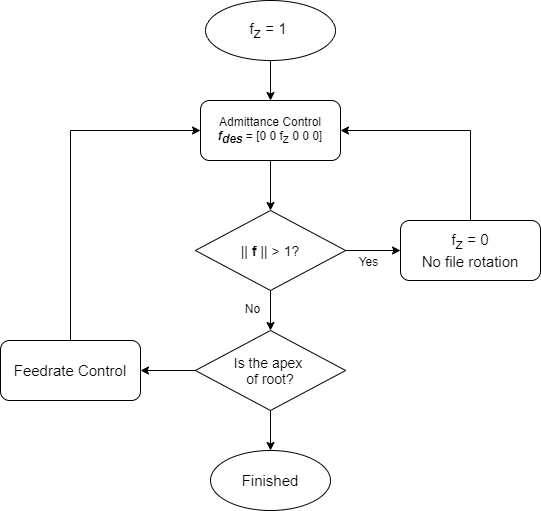
\includegraphics[width= 1\linewidth]{Images/feedrate_control_flow_chart.png}
\caption{Flow chart of Feedrate Control with the DentiBot. $f$ represents force vector}
\label{fig: feedrate_control_fc}
\end{center}
\end{figure}

\section{Automated Endodontic Treatment}
\hspace*{6mm}After pre-clinical evaluation, we found that cleaning root only with force-guided alignment and feedrate control is impracticable. The endodontic file is easy to get stuck in the root due to root debris. Once the stuck happens, the file torque will increase dramatically. File feedrate control can not handle the dramatic increase. The effective way to solve this problem is to rotate inverse the file. Because it is essential to withdraw to get rid of root debris cut by file. The new idea that combines for-guided alignment, inverse rotation control, and file feedrate control is proposed.
\begin{figure}[htbp]
\begin{center}
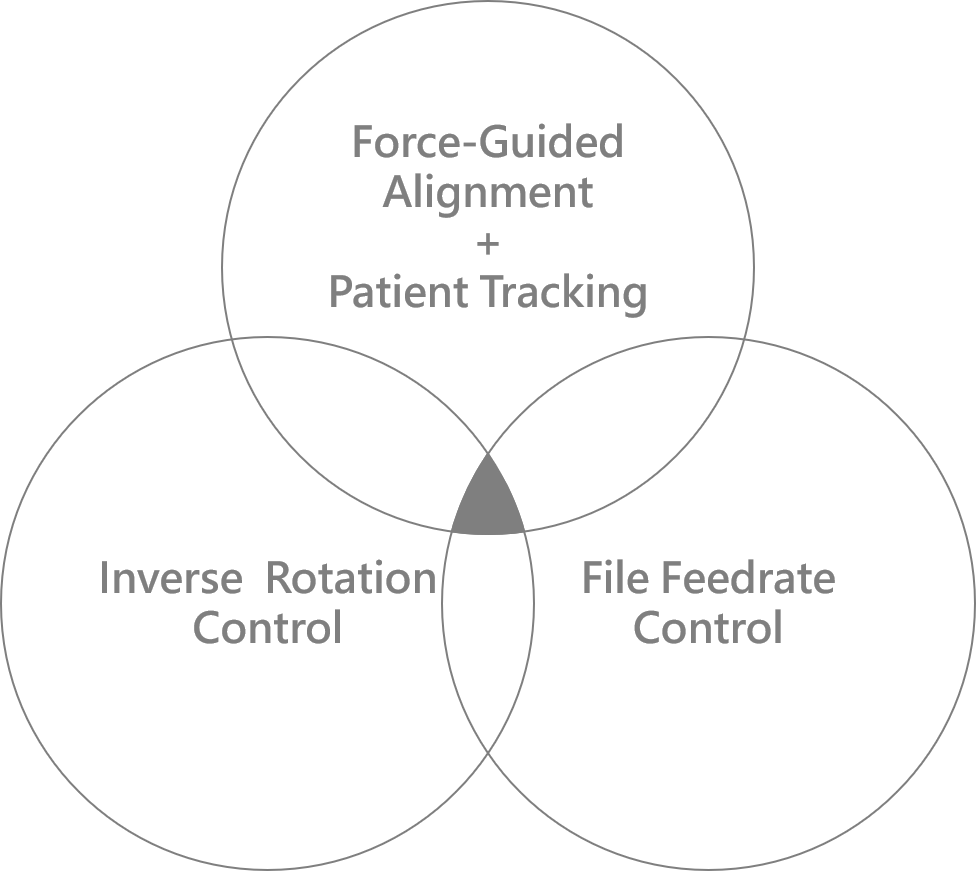
\includegraphics[width=0.7\linewidth]{Images/combine.png}
\end{center}
\caption{Methods of Automated Endodontic Treatment}
\label{fig: combine}
\end{figure}
\par
In view of this, a new algorithm for automated endodontic treatment that combines for-guided alignment, inverse rotation control, and file feedrate control  is proposed as shown in Fig \ref{fig: complete_flowchart}.
\begin{figure}[htbp]
\begin{center}
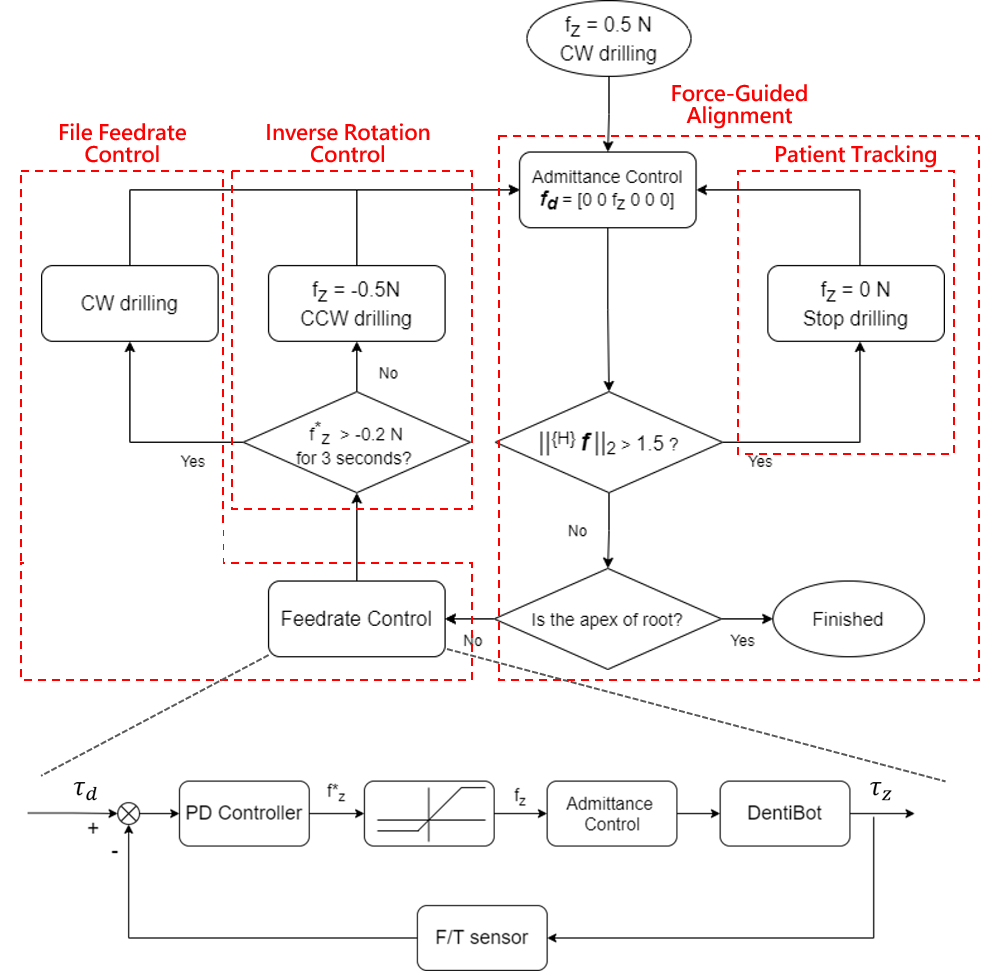
\includegraphics[width=1\linewidth]{Images/algorithm.png}
\end{center}
\caption{
Algorithm for robot-assisted endodontic treatment
}\label{fig: complete_flowchart}
\end{figure}
\par
 Based on the flow chart of feedrate control in Fig \ref{fig: feedrate_control_fc}, inverse rotation control is involved as shown in the left part. The minimum and maximum saturation is from $-0.5$ to $0.5$. When the file torque exceeds the desired torque, Feedrate control will slow down the feed by output $f^*_z$ with a negative value. If  the file torque exceeds a little and $f^*_z$ does not reach $-0.2$, the file will keep clockwise drilling. The above function is essential because it provides the feedrate control a feasibility to regulate the torque.  On the contrary, once the file torque exceeds much and  $f^*_z$  is smaller than $-0.2$, it will trigger the inverse rotation control. That means the file torque increases dramatically so that the feedrate control can not handle with. 
